\section{Specification of Buddy Allocation Model}\label{sec:spec}
The specification of the buddy memory allocation consists of a model for the necessary data structures to represent the memory layouts, as well as the allocation and disposal operations. This specification follows the algorithms for the buddy memory management in Zephyr OS, which applies a quartering split over blocks.

\subsection{State Representation}
\label{statedes}
{In the specification, the state models the memory as a set of  quad-tree each of them representing a memory pool. At this level of the specification, we assume that applications work with our block entity, so requesting a memory block returns the block itself, which will be used later during the deallocation.}
\begin{align*}
&(set:\ 'a)\ tree\ =\ Leaf\ (L:\ 'a)\ | \\
&Node\ (LL:\ 'a\ tree)\ (LR:\ 'a\ tree)\ (RL:\ 'a\ tree)\ (RR:\ 'a\ tree)
\end{align*}

We define the structure of a quad-tree inductively. A quad-tree is parametrized by a variable type $'a$ and it has two constructors: \emph{Leaf} and \emph{Node}. {A \emph{Leaf} is a terminal node storing values of the parametrized type $'a$, and a \emph{Node} has four (sub)trees that are built recursively.} Notations \emph{LL}, \emph{LR}, \emph{RL} and \emph{RR} return the corresponding subtrees of the \emph{Node} tree. Notation \textbf{set} {represents} a function that \mycomment{there is not a more natural way to write the following expression? how a function \textit{gathers [a/the] polymorphic notation?}, rewrite using normal senteces}gathers polymorphic notation \emph{'a} as a collection from all Leaf nodes.

In this specification, we use the tuple (\emph{block\_state\_type} $\times$ \emph{ID}) to instantiate the polymorphic {type} \emph{'a} in the quad-tree structure. Type \emph{block\_state\_type} {indicates} the usage state of a block {and it is constructed using an Isabelle/HOL \emph{datatype}}. It consists of two subtypes{:} \emph{ALLOC} and \emph{FREE} {The former is used to mark memory blocks that have been allocated to applications, whilst the latter is used to mark those unallocated blocks (hence they are free to be assigned to applications requesting memory)}. {The type \emph{ID} is a natural number representing the} address identifier of a memory block. Finally, type \emph{BlockTree} represents an instantiated quad-tree {in which terminal nodes represent allocated or free memory blocks identified with by a natural number. We will use indistinctively the terms of Leaf and memory block along the document}. Non terminal nodes \emph{Node} represent the splitting process of the algorithm. 
{\footnotesize
	\begin{align*}
	block\_state\_type\ &=\ FREE\ |\ ALLOC \\
	ID\ &=\ nat \\
	BlockTree\ &=\ (block\_state\_type\ \times\ ID)\ tree
	\end{align*}
}

{The allocation and free services are defined as a number of operations over the \emph{quad-tree} data structure representing the memory. These operations manipulate a \textsl{BlockTree}, accessing and modifying its structure and the data it stores}. Function \textbf{get\_level} takes{two \emph{BlockTree}, \emph{btree} and \emph{b}}, {and it returns a natural number \emph{level}} {that} represents the layer number {where} \emph{b} {is located} in \emph{btree} from the root node. {The level of a node with regards to itself is $0$, and if the \emph{blocktree} $b$ does not belongs to $btree$ the function also returns $0$.}  Functions \textbf{allocsets} and \textbf{freesets} take a \emph{BlockTree} \emph{btree} and returns a \emph{BlockTree} set \emph{aset} of all the Leaf nodes from \emph{btree} whose \emph{block\_state\_type} are well \emph{ALLOC} for the function \textbf{allocsets}, well \emph{FREE} for the function \textbf{freesets} \mycomment{the comma totally change the meaning of the sentence. With the comma you are saying that all leaf nodes from btree are ALLOC. To express what you wanted to say you need to remove the comma} \mycomment{Since both functions are similar it is better to put them together}. Function \textbf{freesets\_level} takes a \emph{Blocktree} \emph{btree} and a natural number $l$, and it returns a set with all the free Leaf nodes located at level $l$ in \emph{btree}. We use {the} notation \emph{idset} to represent the collection of all used \emph{IDs}. To create a new Leaf node, we {pick up as new leaf \emph{ID} any natural number not belonging to \emph{idset}}.

%Before introducing allocation model, we create a function \textbf{output\_level} \correct{that maps requested size to the allocation level in a quad-tree}{mapping levels of a }. The input parameters are a natural list \emph{blo\_list} and a natural \emph{rsize}. Static linked list \emph{blo\_list} is used to store all possible sizes of blocks in a quad-tree, and its indexes represent the levels of blocks located in this quad-tree. For example, the size of root node is 1024\emph{Mbytes} and the first level of quad-tree is 256\emph{Mbytes}, then \emph{blo\_list}!0 is equal to 1024 and \emph{blo\_list}!1 is 256. The \emph{blo\_list} is a strictly decreasing list to simulate the fact that the smaller the level is, the larger size the memory block owns. This function returns a natural index \emph{l} in \emph{blo\_list} with these constrains: the size it represents has to be greater than or equal to the size of requested block, and there is no smaller size that meets this condition. After that, the block size is picked up from \emph{blo\_list}, and then mapped to the correct level of the quad-tree by the index \emph{l} in \emph{blo\_list}. We use \emph{rlv} to represent the output. The definition of this mapping is as follows.

%\begin{definition} [Mapping Requested Size to Allocation Level]
%\label{mostsuitable}
%\end{definition}
%{\footnotesize
%\begin{align*}
%&output\_level\ blo\_list\ rsize \triangleq THE\ l.\ l < \vert blo\_list \vert \\
%&\wedge rsize \le blo\_list\ !\ l \\
%&\wedge ((\vert blo\_list \vert > 1 \wedge l < \vert blo\_list \vert - 1) \longrightarrow rsize > blo\_list\ !\ (l+1))
%\end{align*}
%}

\subsection{Allocation Model}

The allocation takes as input a set of quad-trees representing the available memory pools $bset$, and a natural number $s$ representing the requested size of the memory to allocate. If $s$ is bigger than the maximum size $\Omega$ for any memory pool then the allocation fails and the state is not modified. If $s$ is smaller or equal than $\Omega$, then it calls function \textbf{alloc} over $bset$ and the level $rlv$ containing blocks of size bigger or equal to $s$, given by $\Delta_s$ as defined in Section~\ref{sec:buddy}. \textbf{alloc} carries out the necessary operations to find a block of size bigger or equal than $s$, and conducts the necessary modifications on $bset$ as we describe below. 

We explain first functions that \textbf{alloc}  uses to obtain the level on a system with free blocks with capacity to allocate a requested size: \textbf{exists\_freelevel} and \textbf{freesets\_maxlevel}. We first provide a description of these functions. Function \textbf{exists\_freelevel} is a predicate taking as input a set of \emph{BlockTree} $bset$ (the collection of all quad-trees in memory system) and a natural number $rlv$, and returns true if there exist a \emph{BlockTree} $b\in bsets$ and a level $l$ in $b$ such that $l$ has at least a free node. Function \textbf{freesets\_maxlevel} has the same inputs, and it returns the maximum level less or equal than \emph{rlv} having at least a free node. Formally:

\begin{definition} [Existence of Free Leaf Nodes]
\end{definition}
\vspace{-7pt}
{\footnotesize
\begin{align*}
exists\_freelevel\ bset\ rlv &\triangleq \exists l.\ l \leq rlv \\
&\wedge \exists b \in bset.\ freesets\_level\ b\ l \ne \emptyset
\end{align*}
}
\vspace{-12pt}

\begin{definition} [Maximum Level of Free Leaf Nodes]
\end{definition}
\vspace{-7pt}	
{\footnotesize
\begin{align*}
&freesets\_maxlevel\ bset\ rlv \triangleq THE\ lmax.\ lmax \leq rlv \\
&\wedge \exists b \in bset.\ freesets\_level\ b\ lmax \neq \emptyset \\
&\wedge (\forall l \leq rlv.\ \exists b \in bset.\ freesets\_level\ b\ l \ne \emptyset \longrightarrow l \leq lmax)
\end{align*}
}
\vspace{-12pt}

During the allocation process, if there is not any free \emph{Leaf} node available at the best fit level $l$ for the requested size, but there exists a higher level $hl \geq l$ with free blocks, it is necessary to start the splitting process from $hl$ down to $l$. Function \textbf{split} recursively divides  $hl - l$ times a Leaf node \emph{b} into a Node tree \emph{btree}. It uses the function \textbf{divide} that takes a Leaf node \emph{b} and returns a new non-terminal Node tree \emph{n} with four terminal Leaf nodes. The division operation is always conducted on the leftmost subtree of $n$ marking it as allocated, while the rest are marked as \emph{FREE}. A simple example describing this process is shown in Fig.~\ref{fig:splitleaf}. We define the \emph{split} operation as follows.

\begin{figure*}[htbp]
	\centering
	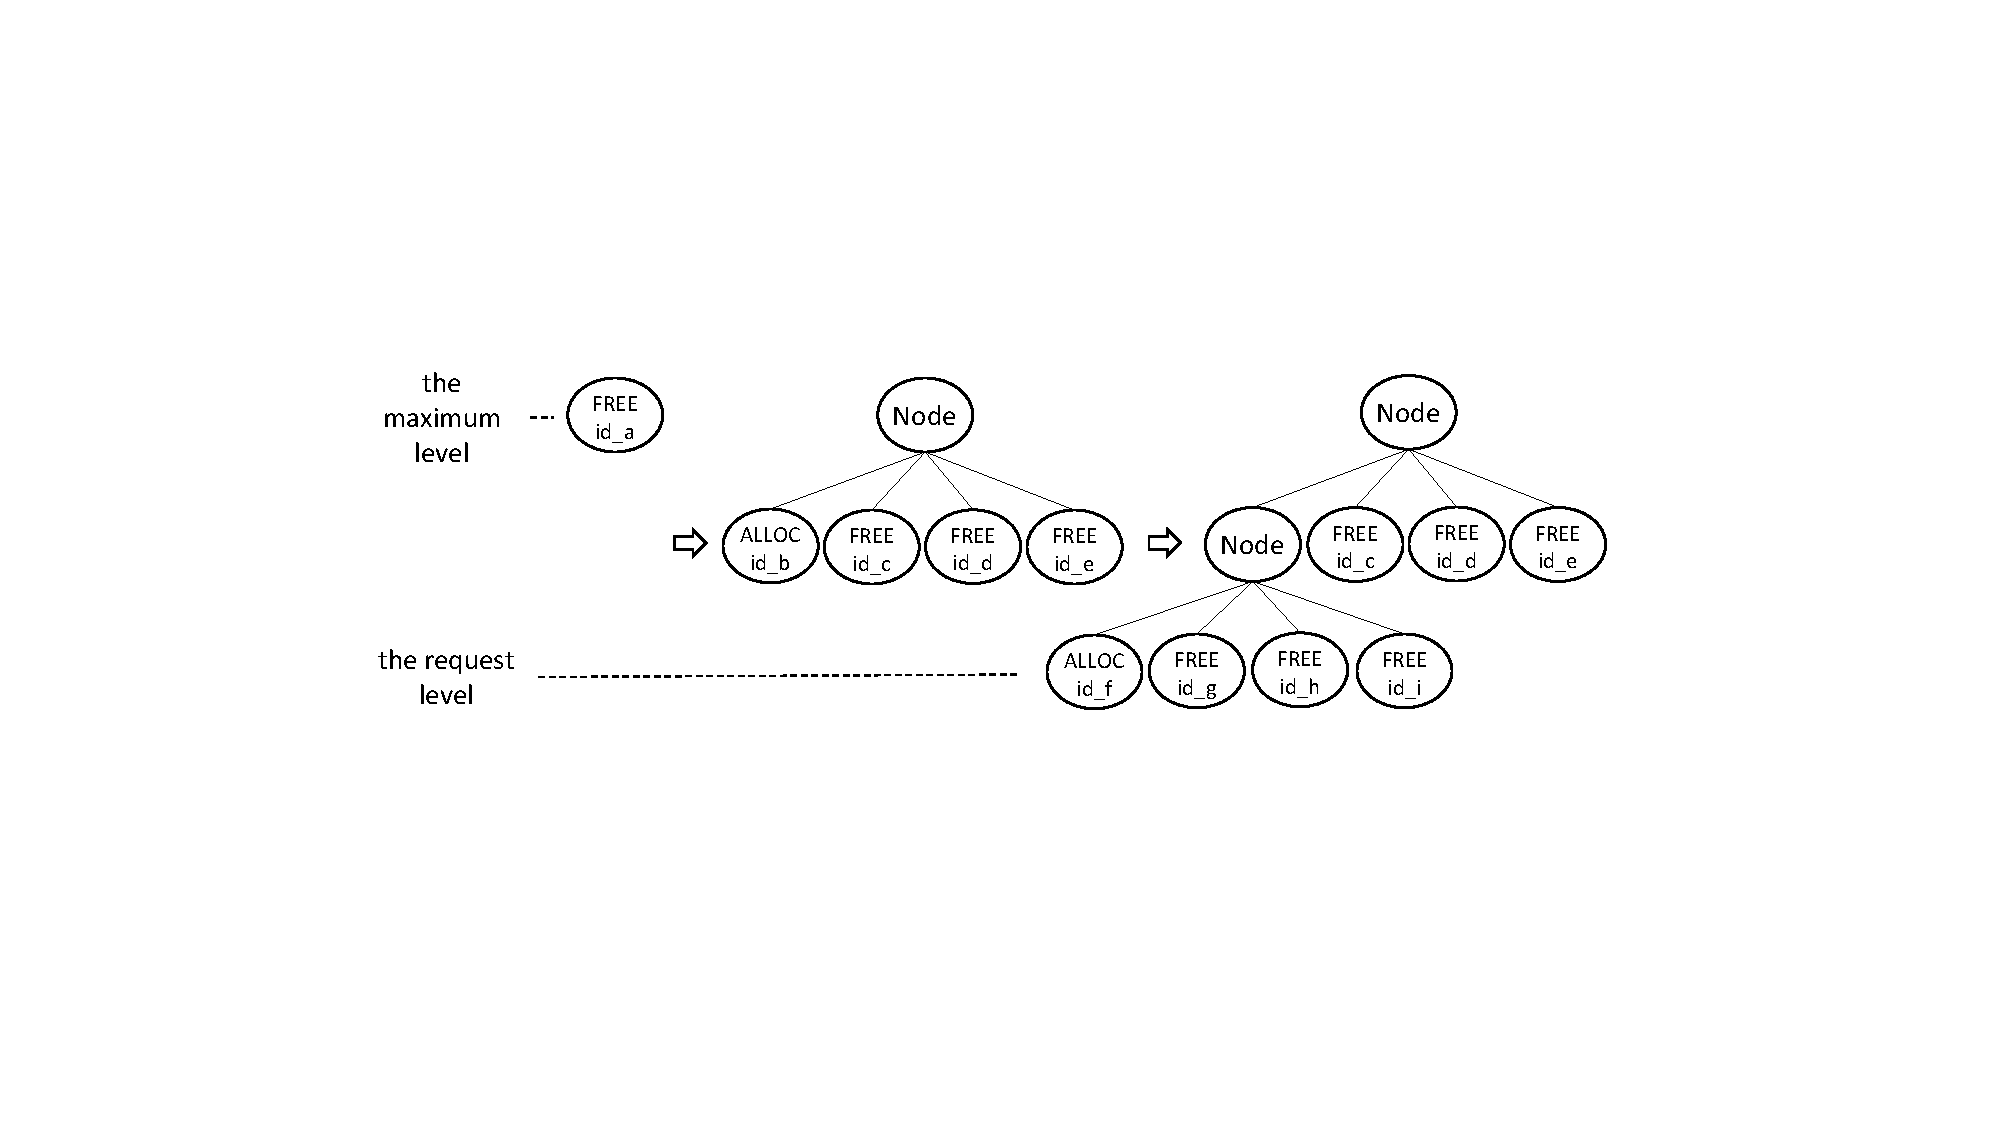
\includegraphics[width=0.9\textwidth]{fig1.pdf}
	\caption{The progress of dividing a free leaf}
	\label{fig:splitleaf}
\end{figure*}

\begin{definition} [Split a Leaf Node]
\end{definition}
\vspace{-7pt}
{\footnotesize
\begin{align*}
split\ b\ lv \triangleq\ &if\ lv = 0\ then\ b \\
else\ Node\ &(split\ (LL\ divide\ b)\ (lv - 1))\ (LR\ divide\ b)\\ 
&(RL\ divide\ b)\ (RR\ divide\ b)
\end{align*}
}	
\vspace{-12pt}

In addition, the allocation use functions \textbf{set\_type}, \textbf{replace} and \textbf{replace\_leaf}. Function \emph{set\_type} takes a Leaf node \emph{b} and a target \emph{block\_state\_type} \emph{s} as inputs, and returns a leaf \emph{b'} resulting of changing the state of \emph{b} to \emph{s}. Function \emph{replace} takes a \emph{BlockTree} \emph{btree}, two Leaf nodes \emph{b} and \emph{b'} as inputs, and returns a tree replacing the Leaf node \emph{b} with \emph{b'} in \emph{btree}. Function \emph{replace\_leaf} takes a \emph{BlockTree} \emph{btree}, a Leaf node \emph{b} and a Node \emph{btr} as inputs, and returns the tree that replaces the Leaf node \emph{b} with \emph{btr} in \emph{btree}.


To allocate a block of size $s$ as described in Section~\ref{sec:buddy}, \textbf{alloc} firstly uses the function \emph{exists\_freelevel} to check whether there is a \emph{BlockTree} in \emph{bset} with free blocks in a a level $l \leq \emph{rlv}$. If there is not, then the allocation process fails and returns original \emph{bset}.  Otherwise, the function \emph{freesets\_maxlevel} returns the maximum level $lmax$ with $lmax \leq rlv$ containing free blocks. From here there are two options.

(a) there is a \emph{BlockTree} with free nodes at the requested level (hence\emph{lmax} is equal to thee requested level \emph{rlv}). In this case the allocation operation selects a \emph{BlockTree} \emph{btree} from $btree$ such that there are free blocks at level \emph{rlv}. After this, it randomly picks up a \emph{FREE} Leaf node \emph{l} in level \emph{rlv} from \emph{btree}, and obtains a new $btree'$ by modifying in $btree$ the type of \emph{l} as \emph{ALLOC} using the functions \emph{set\_type} and \emph{replace\_btree}. After that, the allocation returns an updated \emph{bset} by replacing the previous \emph{btree} with \emph{btree'}. Note that this execution branch do not adds any additional nodes into the tree structure, and only modifies the type of a terminal node at level \emph{rlv}.

(b) there is not a \emph{BlockTree} with free nodes at the requested level (hence \emph{lmax} is smaller to thee requested level \emph{rlv}). Since  \emph{lmax} is a lower level than \emph{rlv} means that free nodes have bigger size than what is requested. In that case it is necessary to modify the tree splitting a terminal Leaf $l$ at level \emph{lmax} down to level \emph{rlv} to create a block fitting better the requested size. The allocation operation selects a \emph{BlockTree} \emph{btree} from $btree$ such that there are free blocks at level \emph{lmax}. Then it selects randomly picks up a \emph{FREE} Leaf node \emph{l} in level \emph{lmax} from \emph{btree} and splits \emph{l} into a \emph{Node} \emph{btr} using the function \emph{split}. As explained above, \emph{split} \emph{``breaks"} the leaf \emph{l} into a new \emph{BlockTree} for which \emph{btr} is its root, and where there is block $b$ at depth $rlv - lmax$ from $btr$ that is allocated and its buddies are free. \textbf{alloc} then updates \emph{l} with \emph{btr} in  \emph{btree} using \emph{replace\_leaf} obtaining \emph{btree'}, to finally update \emph{bset} by replacing the previous \emph{btree} with \emph{btree'}. Finally, the operation returns updated Block set and \emph{True}.

Note that \textbf{alloc} modifies a free block into an allocated one, so the number of leafs remain unmodified in the branch (a); or breaks a free block into a \emph{Node} to eventually create a number of free blocks and a allocated block as shown in Fig.~\ref{fig:splitleaf}. In both cases the rest of leafs are from the original set do not change and there is a new allocated block that was not present. To obtain the block \textbf{alloc} allocates, it is only necessary to subtract the allocate nodes in the original set of free nodes from the allocate nodes in the resulting set.

\begin{definition} [Allocation Operation]
\end{definition}
\vspace{-7pt}
{\footnotesize
\begin{align*}
alloc\ &bset\ rlv \triangleq \\
&if\ exists\_freelevel\ bset\ rlv\ then \\
&\ \ \ \ lmax = freesets\_maxlevel\ bset\ rlv \\
&\ \ \ \ if\ lmax = rlv\ then \\
&\ \ \ \ \ \ \ \ btree = SOME\ b.\ b \in bset \wedge freesets\_level\ b\ rlv \ne \emptyset \\
&\ \ \ \ \ \ \ \ l = SOME\ l.\ l \in freesets\_level\ btree\ rlv \\
&\ \ \ \ \ \ \ \ btree' = replace\ btree\ l\ (set\_type\ l\ ALLOC) \\
&\ \ \ \ \ \ \ \ return\ (bset - \lbrace btree \rbrace \cup \lbrace btree' \rbrace, True) \\
&\ \ \ \ else \\
&\ \ \ \ \ \ \ \ btree = SOME\ b.\ b \in bset \wedge freesets\_level\ b\ lmax \ne \emptyset \\
&\ \ \ \ \ \ \ \ l = SOME\ l.\ l \in freesets\_level\ btree\ lmax \\
&\ \ \ \ \ \ \ \ btr' = split\ l\ (rlv - lmax) \\
&\ \ \ \ \ \ \ \ btree' = replace\_leaf\ btree\ l\ btr' \\
&\ \ \ \ \ \ \ \ return\ (bset - \lbrace btree \rbrace \cup \lbrace btree' \rbrace, True) \\
&else\ return\ (bset, False)
\end{align*}
}
\vspace{-17pt}

\subsection{Deallocation Model}

The deallocation process takes a block $b$ in a level $l$, and sets the state of $b$ to \emph{FREE}. During the deallocation process, if the state of all the buddies of $b$ is already $free$ and $l$ is not the root node, the buddy nodes are merged to avoid fragmentation. In the merging process, $b$ parent \emph{Node} is transformed into a \emph{Leaf} at level $l-1$ that is set as free, causing all the buddies to be removed from the quad-tree. Hence they are not at level $l$ anymore). The merging process is shown in Fig.~\ref{fig:merginfreeblocks}.

\begin{figure*}[htbp]
	\centering
	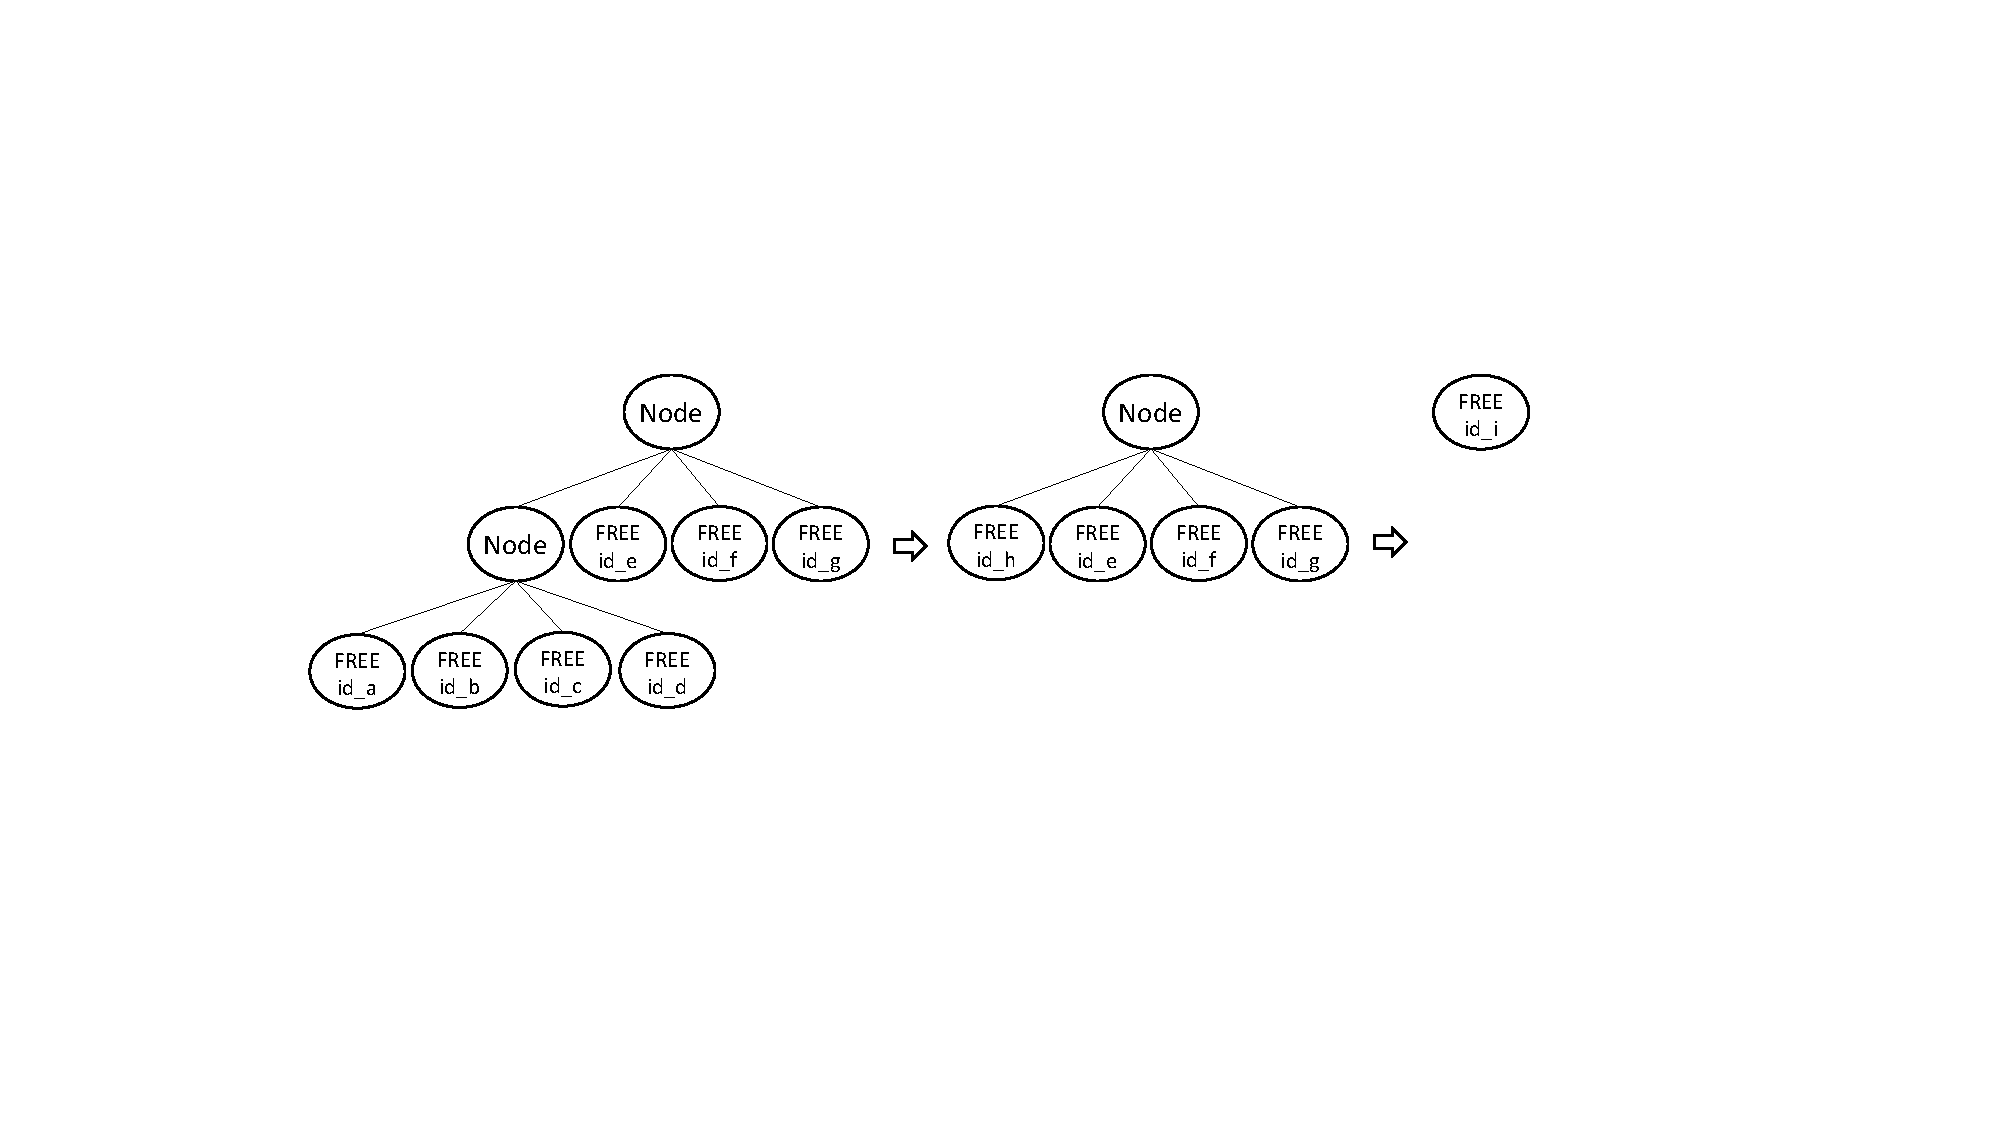
\includegraphics[width=0.9\textwidth]{fig2.pdf}
	\caption{The progress of merging all free memory blocks}
	\label{fig:merginfreeblocks}
\end{figure*}

Function \textbf{free} takes as input a set of \emph{BlockTree} $bset$ and a block to dispose \emph{b}. It firstly checks whether there is a $btree \in bset$ for which \emph{b} belongs to and that its state is \emph{ALLOC}. If the conditions are not met, the procedure fails returning the original \emph{bset}. If they are, the procedure picks up the  tree in \emph{bset} as \emph{btree} to which \emph{b} belongs to, which must be unique. After this, \emph{btree} is modified into \emph{btree'} where the type of \emph{b} is set to \emph{FREE} using the functions \emph{set\_type} and \emph{replace}. After that, the new tree is coalesced using the function \emph{merge} and \emph{bset} is updated replacing \emph{btree} with the new memory pool. The definition of deallocation operation is as follows.

\begin{definition} [Deallocation Operation]
\end{definition}
\vspace{-7pt}
{\footnotesize
\begin{align*}
free\ &bset\ b \triangleq \\
&if\ \exists btree \in bset.\ b \in set\ btree\ then \\
&\ \ \ \ if\ fst\ b = FREE\ then \\
&\ \ \ \ \ \ \ \ return\ (bset, False) \\
&\ \ \ \ else \\
&\ \ \ \ \ \ \ \ btree = THE\ t.\ t \in bset \wedge b \in set\ t \\
&\ \ \ \ \ \ \ \ btree' = replace\ btree\ b\ (set\_type\ b\ FREE) \\
&\ \ \ \ \ \ \ \ btree'' = merge\ btree' \\
&\ \ \ \ \ \ \ \ return\ (bset - \lbrace btree \rbrace \cup \lbrace btree'' \rbrace, True) \\
&else\ return\ (bset, False)
\end{align*}
}
\vspace{-12pt}

At this point, we have finished the specification of the allocation and disposal operations for a buddy memory allocator. The next section tackles the verification of functional and security properties over the model for the allocation and deallocation operations.